This chapter introduces the methodological framework used in this thesis 
and provides an overview of the system developed to investigate the research questions. 
The system developed, called MLguide, is a web-based decision-support tool for machine learning 
method selection and serves as the central artifact in this work. 
Section~\ref{sec:dsr} presents Design Science Research as the overarching framework. 
Section~\ref{sec:system-overview} gives a high-level description of MLguide 
and its main components. 

The methodology is covered in detail across two chapters. 
Chapter~\ref{ch:system-development} describes the design and development of MLguide,
while Chapter~\ref{ch:research-approach} describes the methods used to investigate the research questions through the use of the system.

\section{Design Science Research}
\label{sec:dsr}
This thesis uses Design Science Research (DSR) as its methodological framework, 
following \textcite{peffers2007design_science_research_methodology} and 
\textcite{hevner2004design_science_information_systems_research}. 
DSR is suited for this work because the research questions are investigated 
through the design and use of a software system. 
In DSR, knowledge is gained by building and evaluating an artifact 
\parencite{hevner2004design_science_information_systems_research}. 
The artifact in this thesis is MLguide, a web-based decision-support system 
built to investigate the research questions defined in Chapter~\ref{ch:introduction}.

The DSR process consists of six activities: problem identification, defining objectives, 
design and development, demonstration, evaluation, and communication 
\parencite{peffers2007design_science_research_methodology}. 
These activities are nominally sequential, but iteration is expected. 
After evaluation, the researcher may return to design and development to improve 
the artifact before proceeding \parencite{peffers2007design_science_research_methodology}. 
Figure~\ref{fig:dsr-methodology-overview} shows how these activities map to the structure 
of this thesis.

\begin{figure}[H]
    \centering
    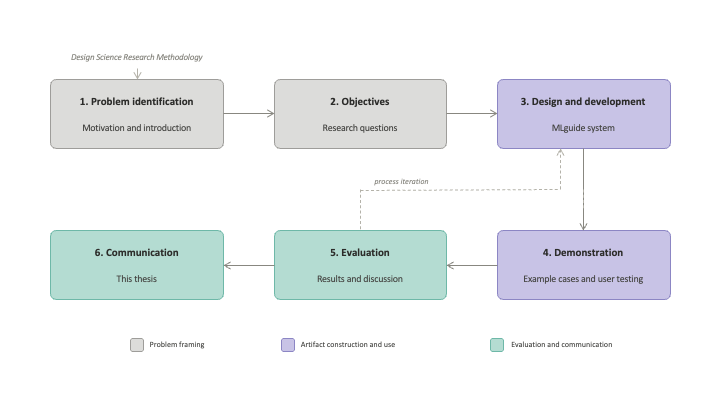
\includegraphics[width=\textwidth]{Figures/dsrm-mlguide.pdf}
    \caption{Design Science Research Methodology inspired by \textcite{peffers2007design_science_research_methodology}}
    \label{fig:dsr-methodology-overview}
\end{figure}

The process in this thesis follows a design-centered initiation, meaning that 
development of the system began before the research questions were fully formalised 
\parencite{peffers2007design_science_research_methodology}. 
This reflects how the work evolved from the pre-master project, where an initial 
roadmap and literature analysis provided the starting point for building MLguide \parencite{bergsto2026mlselection}. 

\section{System Overview}
\label{sec:system-overview}

\begin{figure}[H]
    \centering
    \includegraphics[width=\textwidth]{Figures/mlguide-system-overview.pdf}
    \caption{System Overview of MLguide}
    \label{fig:mlguide-overview}
\end{figure}

This section gives a brief overview of MLguide and its main components.
MLguide is a web-based decision-support system designed to help users select 
machine learning methods for a given problem. 
Figure~\ref{fig:mlguide-overview} gives a high-level overview of the system.

The user starts by describing their problem in a few sentences and can optionally 
provide filters such as ML area, task type, or data type to narrow the scope. 
The system draws on two knowledge sources: a structured ML knowledge base containing 
methods and tasks, and a database of research articles from the literature. 
Based on these inputs, the recommendation engine produces three outputs: 
a ranked list of ML methods, a set of supporting articles from the literature, 
and a starter notebook to support early implementation.